\section{Phase 2}

In the second phase of this project, our goals were to successfully detect lanes, traffic light colors and type, and estimate car poses. We began this section by performing a comprehensive literature review to understand the state-of-the-art techniques for each of these tasks. We then moved forward with the techniques which showed the most promise.


\subsection{Lane Detection}
Given that lane detection was missing feature from our Phase 1, we wanted to get this working as soon as possible. The techniques which provided 3D lane output discussed in the previous section were still not working, so our team looked into more techniques. 

\subsubsection{Other 3D Lane Detection Techniques}
Other lane detection techniques were considered, such as Anchor3DLane \cite{Anchor3DLane}. Again, the same issues with functionality were encountered, and proved too time consuming to resolve. As such our team decided to look into techniques which provided lane output in 2D image space.

\subsubsection{Segmentation of Lane Lines}
The first class of technique that we found in the literature were techniques which segmented the lane lines in an image. The first technique we came across was an extension of YOLO for the express purpose of driving perception, called YOLOPv2 \cite{YOLOPv2}. This network not only segmented the lane lines, but also provided segmentation of other regions, such as drivable area, and also detected vehicles in the scene. The output of this paper on our test data is shown in Figure \ref{fig:YOLOPv2_output}. As is apparent in the image, the lane segmentation was not very precise, which would make it difficult to fit 2D lane lines to the output of this network. Even more problematic, the different lane lines were all classified with the same mask. This was a problem, as our rendering pipeline used Bézier curves to interpolate between a set of sampled points of each lane line separately. This meant that the output of this network was not suitable for our purposes.

\begin{figure}
    \centering
    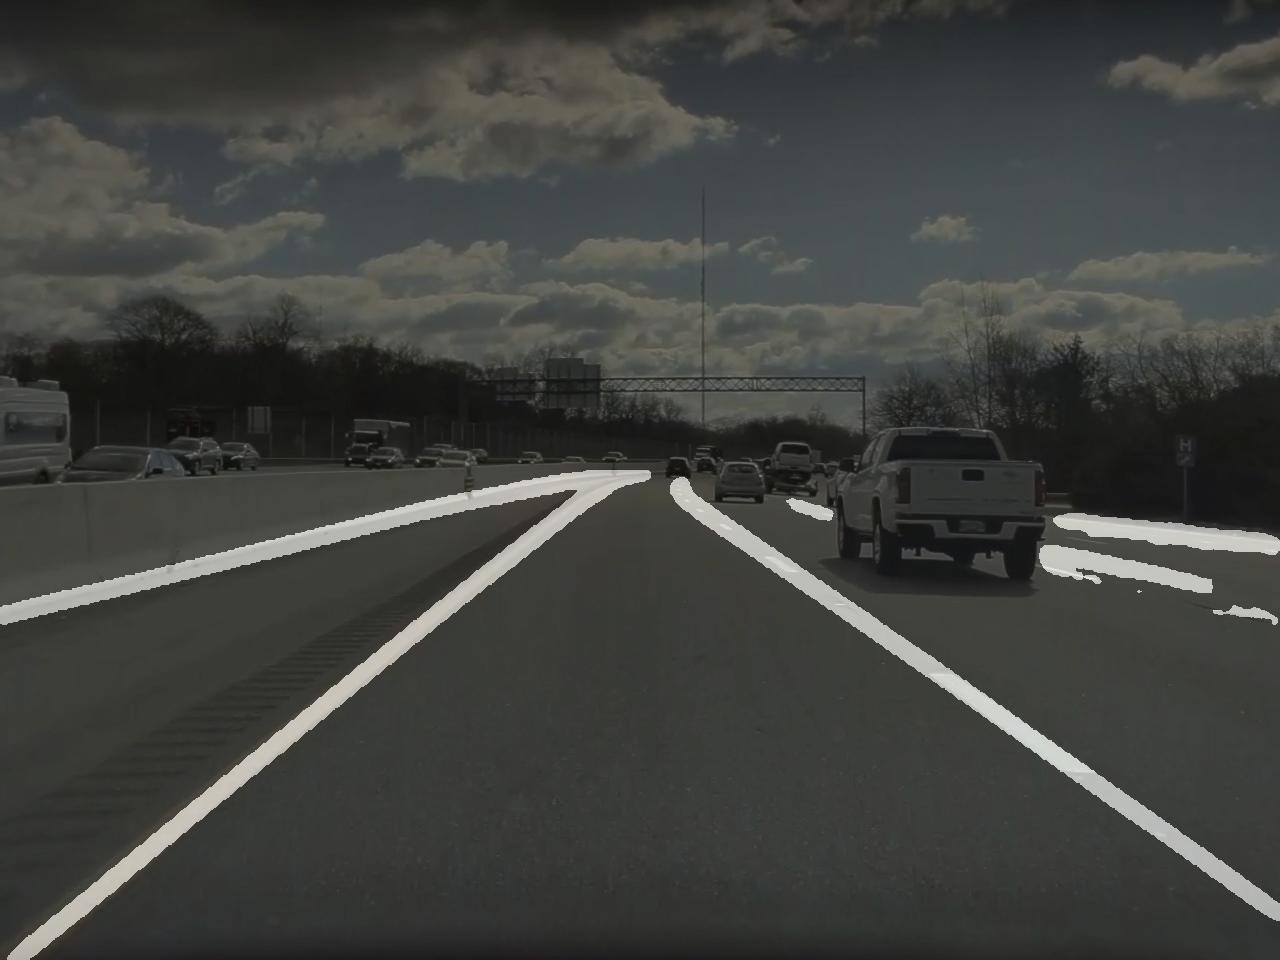
\includegraphics[width=0.9\linewidth]{images/YOLOPv2.jpg}
    \caption{Output of lane detection from YOLOPv2 \cite{YOLOPv2}.}
    \label{fig:YOLOPv2_output}
\end{figure}

Another segmentation technique using a Mask RCNN backbone was considered, but again, the output was not suitable for our pipeline, and the documentation and code for the technique were not as easily available as the YOLOPv2 technique. 


\subsubsection{2D Lane Line Fitting}
The final class of techniques considered would return lane line coordinates fitted to each individual lane line. These techniques were much more useful than the segmentation style 2D detection networks, as we could simply make the assumption that the lanes lay on the ground plane, and project the 2D lane sample points onto the ground plane to recover lane lines. The first technique our team considered was CLRNet \cite{CLRNet}. This network provided decent output, and had documentation on how to run inference with the network on new images. The output of the network is shown in Figure \ref{fig:CLRNet_output}.

Initially, the output of the network was underwhelming, but it was noted that the input images lacked contrast and brightness, and so did not match the training images well. We therefor applied a simple preprocessing step to the images before detecting lanes, which proved effective at improving the output of the network. The output of the network after preprocessing is shown in Figure \ref{fig:CLRNet_output_preprocessed}.

\begin{figure}
    \centering
    \begin{subfigure}{0.95\linewidth}
        \centering
        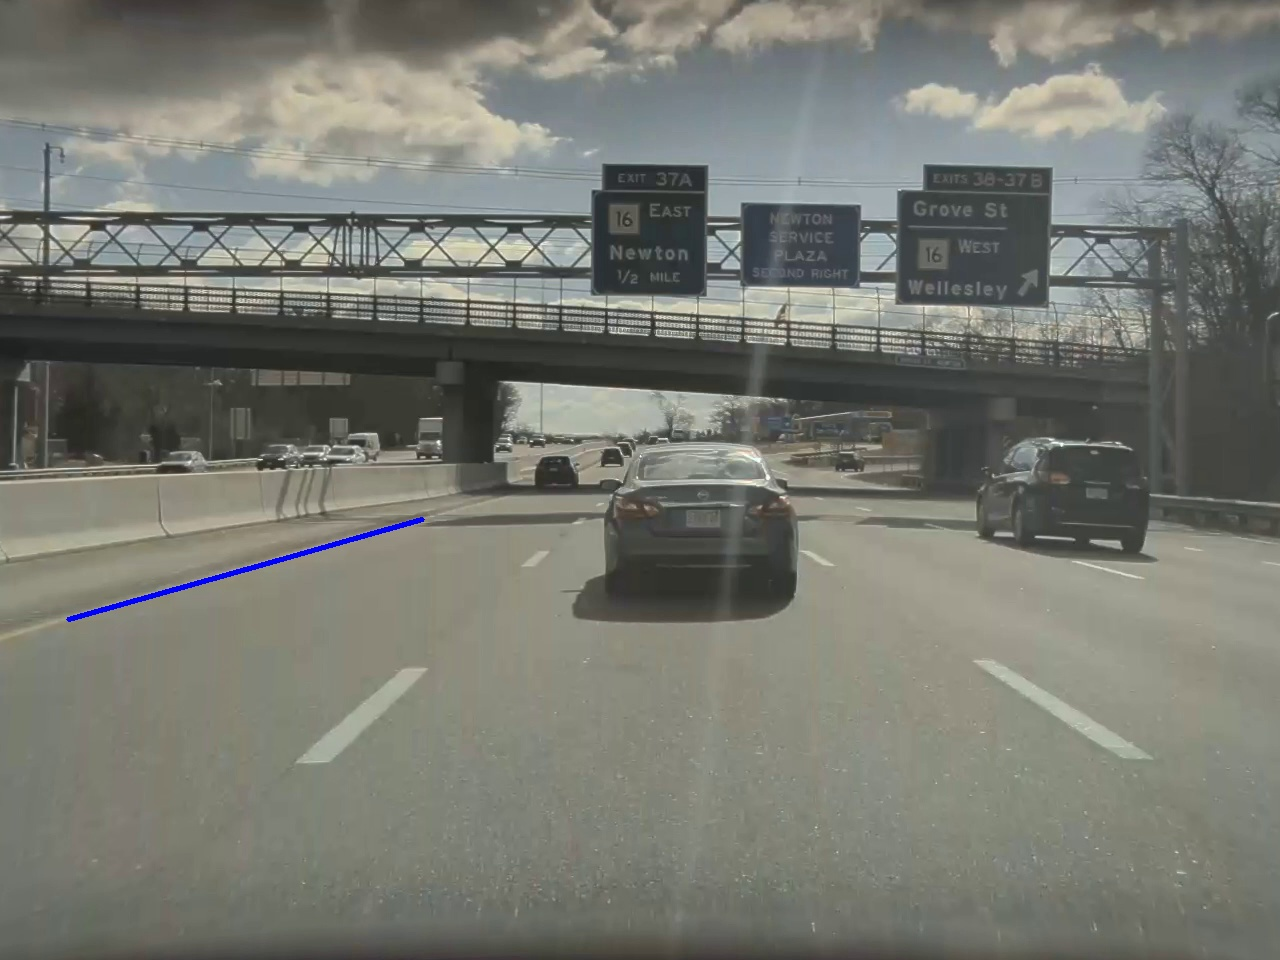
\includegraphics[width=\textwidth]{images/CLRNet_without_proc.jpg}
        \caption{Output of CLRNet before preprocessing.}
        \label{fig:CLRNet_output}
    \end{subfigure}
    \begin{subfigure}{0.95\linewidth}
        \centering
        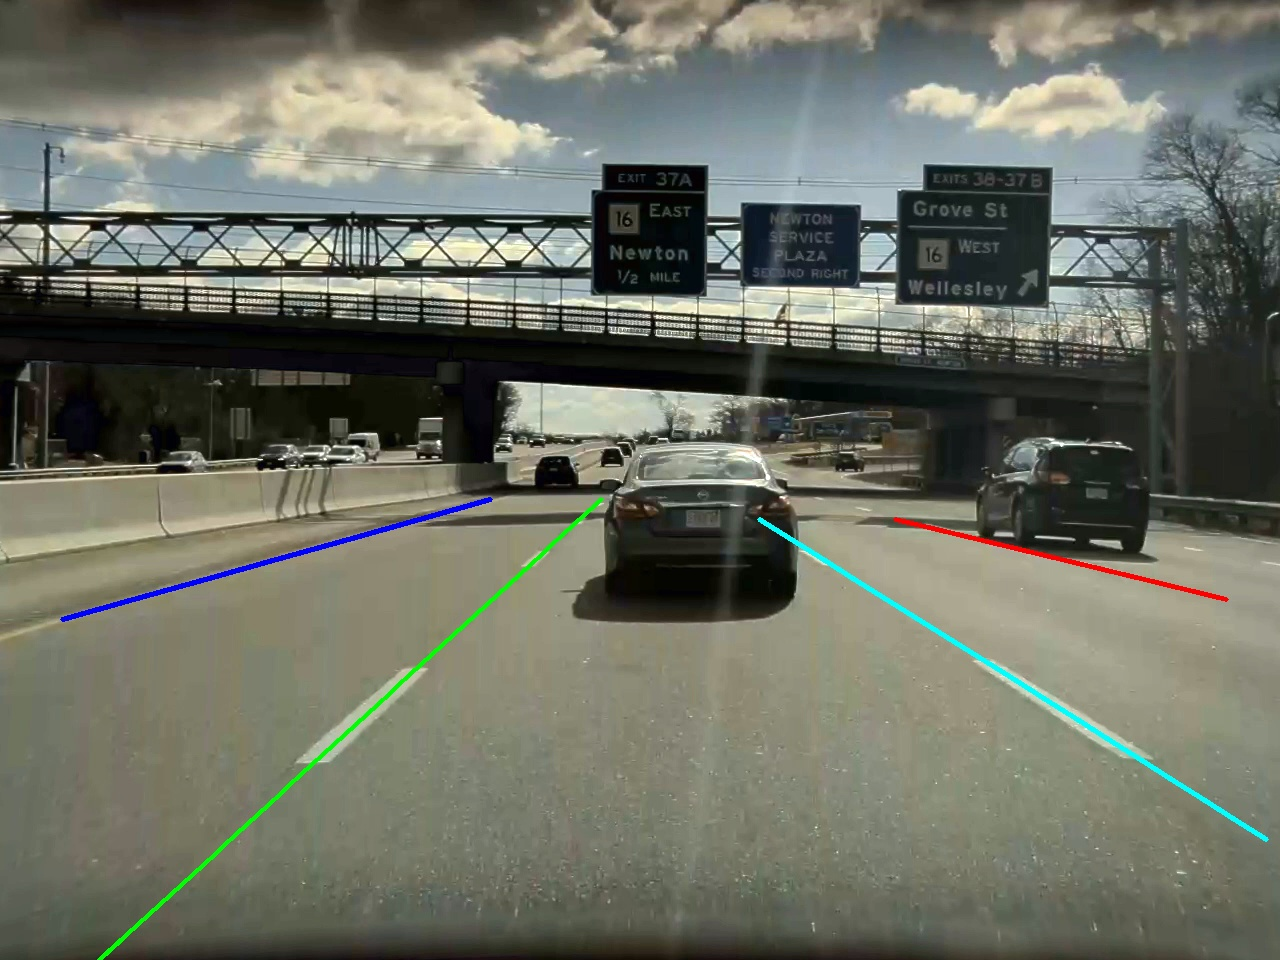
\includegraphics[width=\textwidth]{images/CLRNet_with_proc.jpg}
        \caption{Output of CLRNet after preprocessing.}
        \label{fig:CLRNet_output_preprocessed}
    \end{subfigure}
    \caption{Output of CLRNet \cite{CLRNet}.}
\end{figure}

An extension of CLRNet, discussed in \emph{Recursive Video Lane Detection}, added temporal information to the network greatly improving the consistency of the output on video inputs \cite{RVLD}. Again, the codebase could not be made to function on our test data, and so our team settled on using the CLRNet network for lane detection.

\subsubsection{Lane Line Reprojection}
Once the lane lines were detected, the next step was to re-project the 2D lane lines onto the ground plane. This again began with the pinhole projection model, as described in Equation \ref{eq:pinhole_projection}. We then made the assumption that the camera was looking straight ahead, and that the ground plane was perpendicular to the $XZ$ plane with $Y = -1.5$. This allowed us to simplify the pinhole projection model to the form shown in Equation \ref{eq:simplified_pinhole_projection_2}.
\begin{equation}\label{eq:simplified_pinhole_projection_2}
\begin{aligned}
  \lambda\begin{bmatrix}
    x \\
    y \\
    1
  \end{bmatrix}
  & =
  \mathbf{K}
  \begin{bmatrix}
      \mathbf{I} & \mathbf{0}
  \end{bmatrix}
  \begin{bmatrix}
      X \\
      -1.5 \\
      Z \\
      1
  \end{bmatrix} \\
  \begin{bmatrix}
    X \\
    -1.5 \\
    Z
  \end{bmatrix}
  & =
  \lambda \mathbf{K}^{-1} \begin{bmatrix}
    x \\
    y \\
    1
  \end{bmatrix}
\end{aligned}
\end{equation}
From this equation, we could get the 3D coordinates of the lane lines. The output of the re-projected lane lines is shown in Figure \ref{fig:reprojected_lane_lines}.

\begin{figure}
    \centering
    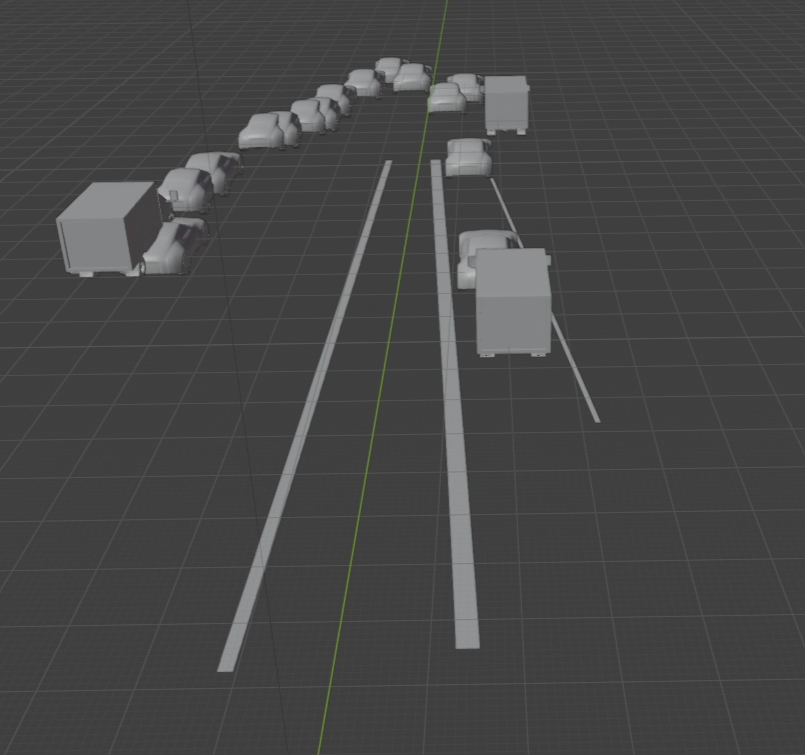
\includegraphics[width=0.95\linewidth]{images/reprojected_lanes.png}
    \caption{Re-projected lane lines.}
    \label{fig:reprojected_lane_lines}
\end{figure}

\subsection{Traffic Light Color Detection}
While the YOLOv9 pipeline from Phase 1 provided 3D localization of traffic lights, it did not provide the color of the traffic light. Our team looked into the literature, and found that some people had fine tuned a YOLO network to detect traffic lights and their colors. We decided to use this technique, as it would fit nicely into our existing pipeline. We used data from cinTA\_v2 dataset to fine tune a YOLOv8 network \cite{CintaV2Dataset}, but the output proved very poor, as detection of traffic lights in the first place was much more inconsistent, and even when detected the color was not correct. Some data manipulation was attempted, such as increasing the contrast, changing the color space, and changing the size of the images, but the output of the fine-tuned networks still remained unusable. Due to time constraints, our team decided to ignore the traffic light color detection for the time being, and focus on the other tasks. Given more time, classical methods would have been pursued using brightness andn some color thresholding to perform the traffic light classification.

\subsection{Car Pose Estimation}
Crucially missing from the first phase of this project was the ability to estimate the pose of the cars in the scene. This was a difficult task, as the only information we had about the cars was their bounding boxes. Many techniques have been proposed over the years, but our team turned back to \emph{3D Bounding Box Estimation Using Deep Learning and Geometry} \cite{3DBoxEstimation}, as it not only provided pose of the object, but also the 3D location. The output of the network on data from the dataset the network was trained on is shown in Figure \ref{fig:3DBoxEstimation_output_trained}, and the output of the network on our test data is shown in Figure \ref{fig:3DBoxEstimation_output_test}. As is apparent from the comparison, the network did not generalize well to our test data, or some other issue was present. This failure, along with the fact that networks which predicted both bounding box and pose would preclude the use of the YOLO pipeline, prompted out team to look into other techniques for car pose estimation.

\begin{figure}
    \centering
    \begin{subfigure}{0.95\linewidth}
        \centering
        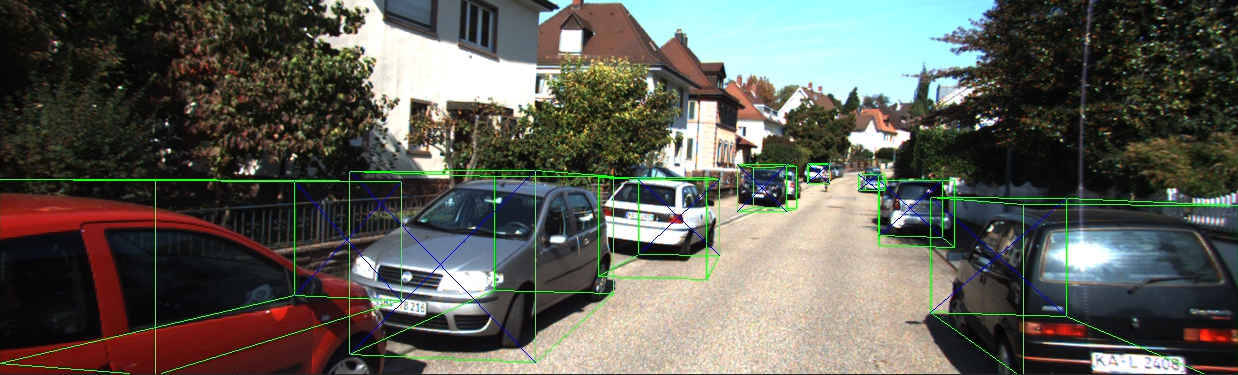
\includegraphics[width=\textwidth]{images/car_pose_train.png}
        \caption{Output on training data.}
        \label{fig:3DBoxEstimation_output_trained}
    \end{subfigure}
    \begin{subfigure}{0.95\linewidth}
        \centering
        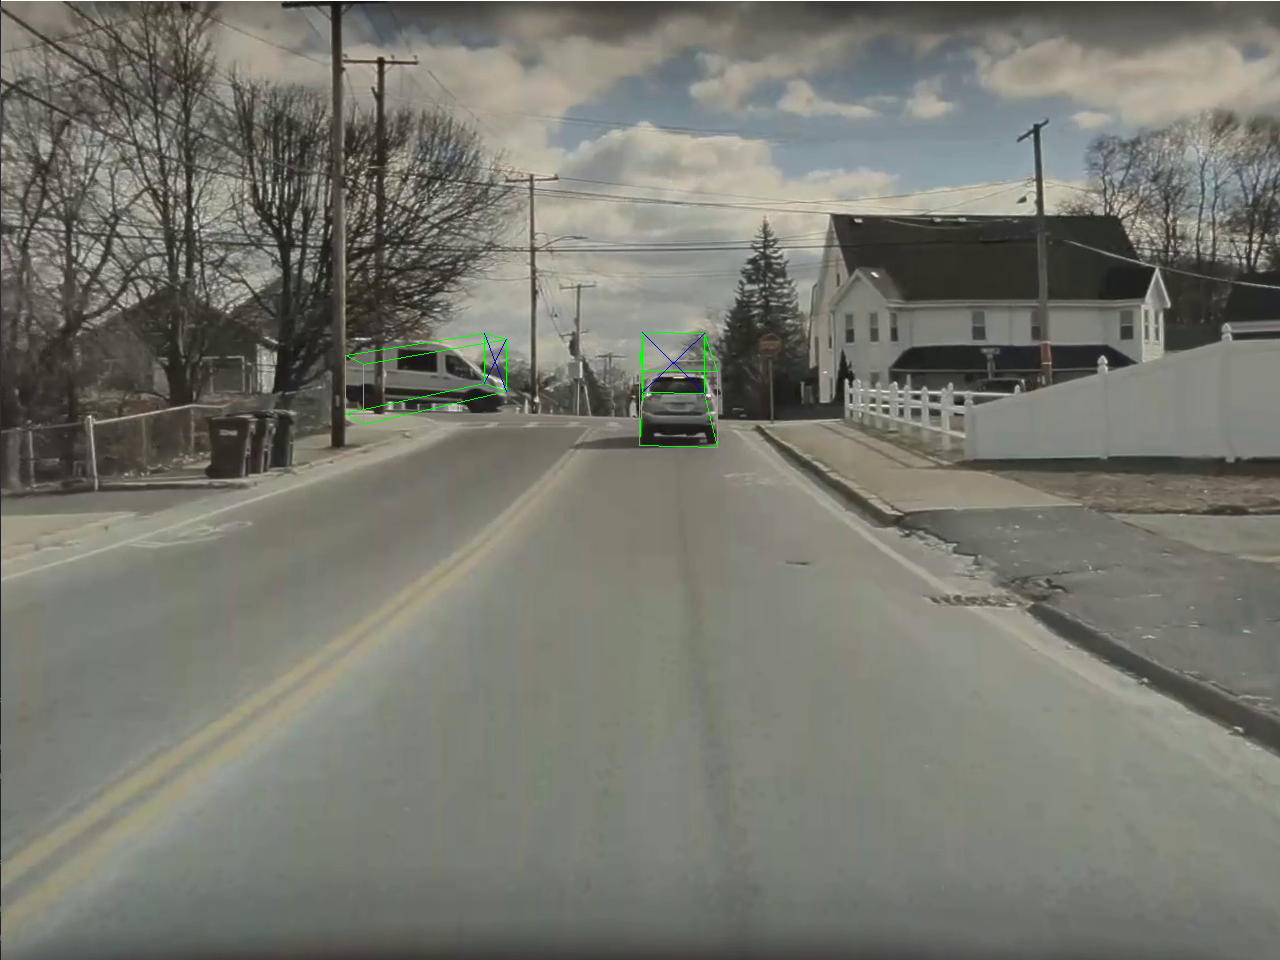
\includegraphics[width=\textwidth]{images/car_pose.png}
        \caption{Output on test data.}
        \label{fig:3DBoxEstimation_output_test}
    \end{subfigure}
    \caption{Output of 3D Bounding Box Estimation Using Deep Learning and Geometry \cite{3DBoxEstimation}.}
\end{figure}

The next technique which our team looked into was called EgoNet \cite{EgoNet}, which had the advantage that it could take in the output of the YOLOv9 network, and then predict the pose of the cars in the scene. The network also came with pre-trained weights, necessary due to our time constraints, but again the code base failed to have good support or documentation on how to run inference on new images. Due to these issues, our team did not include any pose estimation in our pipeline for Phase 2.
